\renewcommand{\vec}[1]{\textbf{#1}}

\chapter{Experimental Results}
\label{cha:experimental_results}

\section{2D Density Estimation}

To test the simple model from Section \ref{sec:simple_pc} with the discussed algorithms, so Expectation Maximization (EM), 
Gradient Descent (GD), Score Matching (SM) and Sliced Score Matching (SSM) from subsections \ref{sec:gmm_em} to \ref{sec:gmm_ssm}, we used some 
two dimensional data to perform density estimation. 

Samples from the three datasets we used can be seen in Figure \ref{fig:2d_datasets}. \\

\vspace{10pt}
\begin{figure}[H]
    \centering
    \begin{subfigure}[b]{0.4\textwidth} 
        \centering
        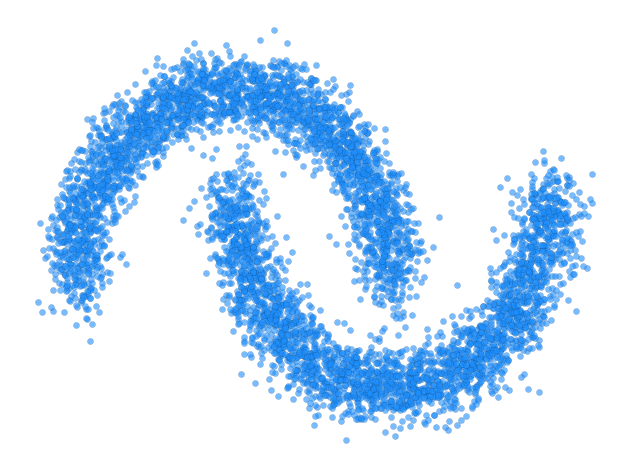
\includegraphics[width=\textwidth]{figures/halfmoons.png}
        \caption{halfmoons}
    \end{subfigure}
    \hfill
    \begin{subfigure}[b]{0.4\textwidth} 
        \centering
        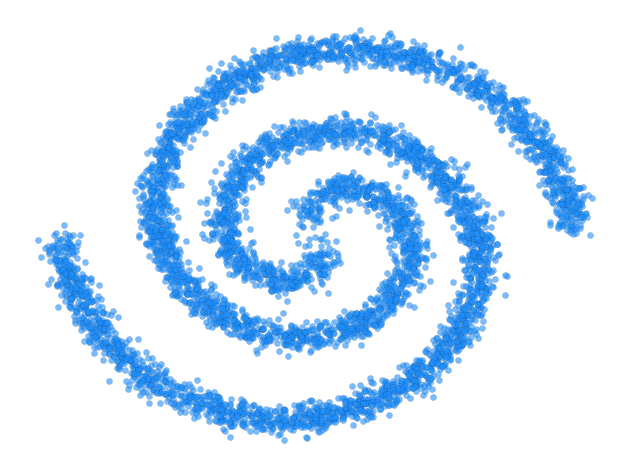
\includegraphics[width=\textwidth]{figures/spirals.png} 
        \caption{spirals}
    \end{subfigure}
    
    \vskip\baselineskip 
    \begin{subfigure}[b]{0.4\textwidth} 
        \centering
        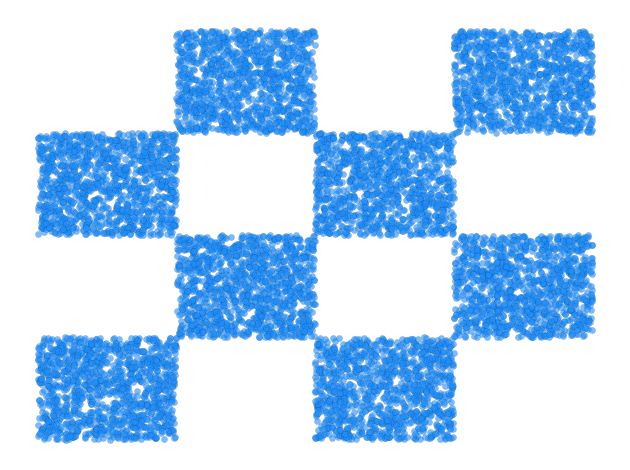
\includegraphics[width=\textwidth]{figures/board.png}
        \caption{board}
    \end{subfigure}
    
    \caption{Samples for all three datasets}
    \label{fig:2d_datasets}
\end{figure}


\subsection{Best Possible Results}

In the basic first set of experiments we wanted to see the best possible results for each algorithm on each dataset. 

For each dataset we generated 20,000 data points and split them evenly for training and validation. However before the training process can start, recall 
that our model is governed by the learnable parameters $\boldsymbol \pi$ (mixture weights), $\boldsymbol \mu$ (means of components) and
$\boldsymbol \Sigma$ (covariance matrices of components) that need to be initialized in some manner and the hyperparameter $K$ (mixture count) that needs to be chosen. 

As for the learnable parameters, we initialized the mixture weights $\boldsymbol \pi$ uniformly 
\[
    \boldsymbol{\pi}_k = \frac{1}{K}, \quad k = 1, 2, \dots, K
\]
the covariance matrices $\boldsymbol \Sigma$ as identity matrices of size $D \times D$ 
\[
    \mathbf{\Sigma}_k = \mathbf{I}_D, \quad k = 1, 2, \dots, K
\]
where $D$ is the dimensionality of the data and the means $\boldsymbol \mu$ by computing cluster centers of the data with the sklearn \cite{sklearn} implementation of KMeans. 

As for $K$, trough some initial testing we chose three different values, namely a minimal $K$, that is needed for producing reasonable results, 
a very large $K$ from which onward there are diminishing returns and a moderate $K$ in the middle between the minimal and the large $K$.

Now for the training process also recall that it is governed by the hyperparameter number of iterations $T$ for all algorithms and 
the hyperparameter learning rate $\eta$ for all the gradient-based algorithms (GD, SM, SSM).
To choose these parameters we fixed $K$ to one of the three chosen values and did cross-validation by computing the validation set Log-Likelihood 
of the models with all possible remaining hyperparameter combinations and choosing the combination with the highest Log-Likelihood.

Results, more specifically Log-Likelihood, estimated densities and samples for all datasets and all values of $K$ with the best possible training-specific 
hyperparameters can be seen in the following three pages. Note that when setting the same random seed all of these results should be 
reproducible.

\newpage
\begin{figure}[H]
    \centering
    \makebox[\textwidth][c]{\hspace*{-1cm} 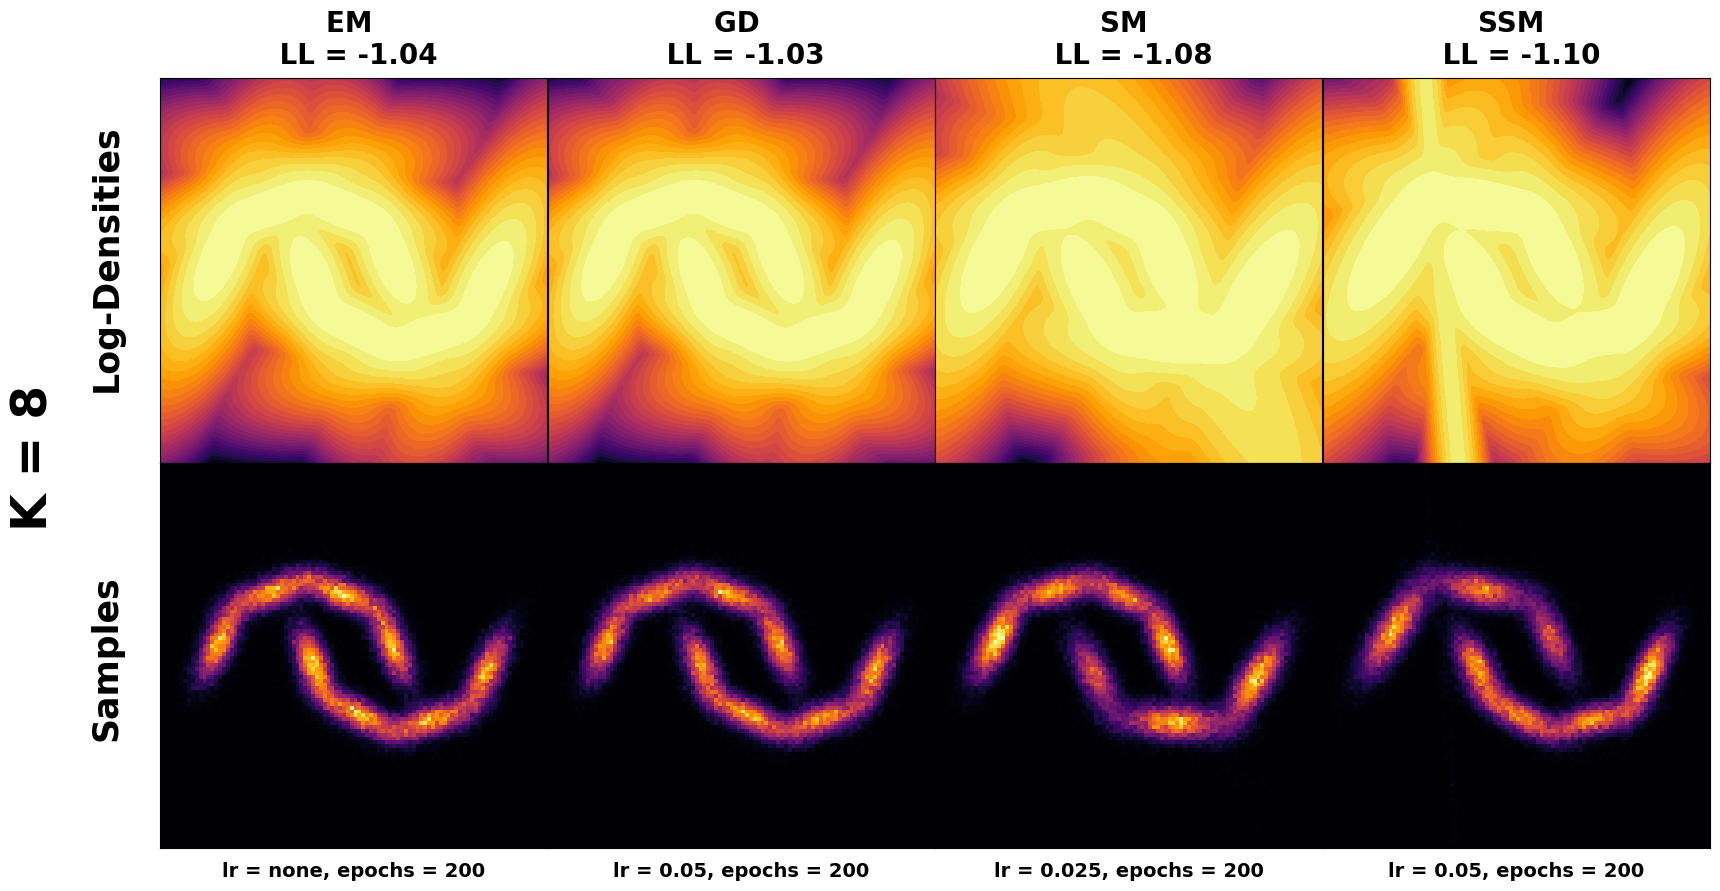
\includegraphics[width=0.9\textwidth]{figures/halfmoons/halfmoons_8.png}}
    \vskip 5pt
    \makebox[\textwidth][c]{\hspace*{-1cm} 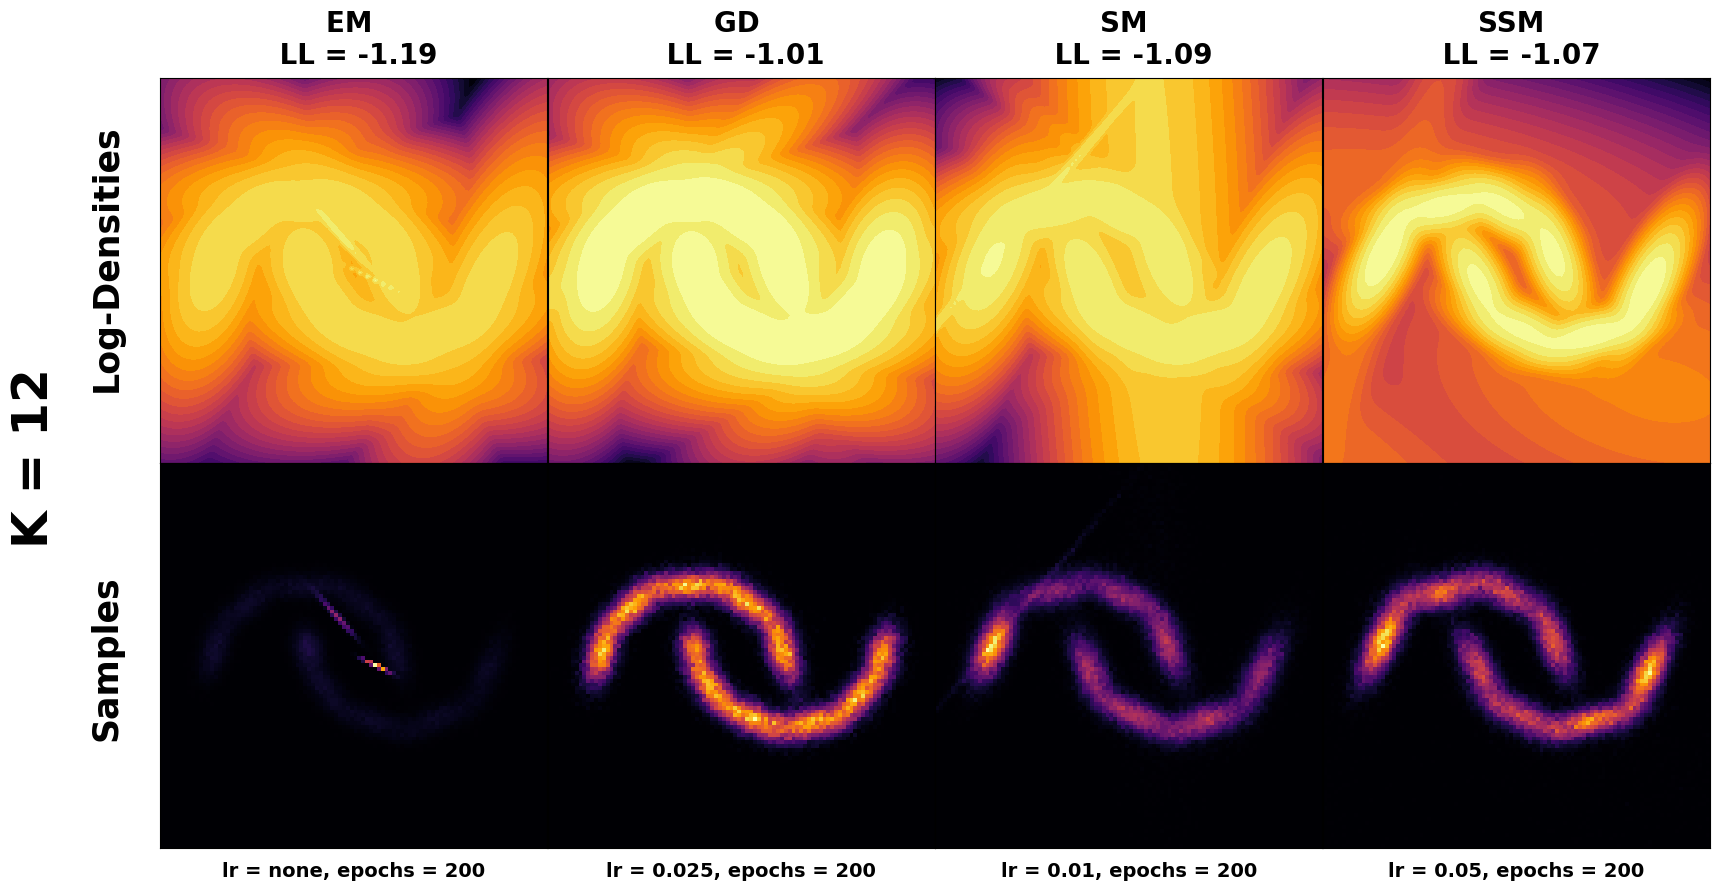
\includegraphics[width=0.9\textwidth]{figures/halfmoons/halfmoons_12.png}}
    \vskip 5pt
    \makebox[\textwidth][c]{\hspace*{-1cm} 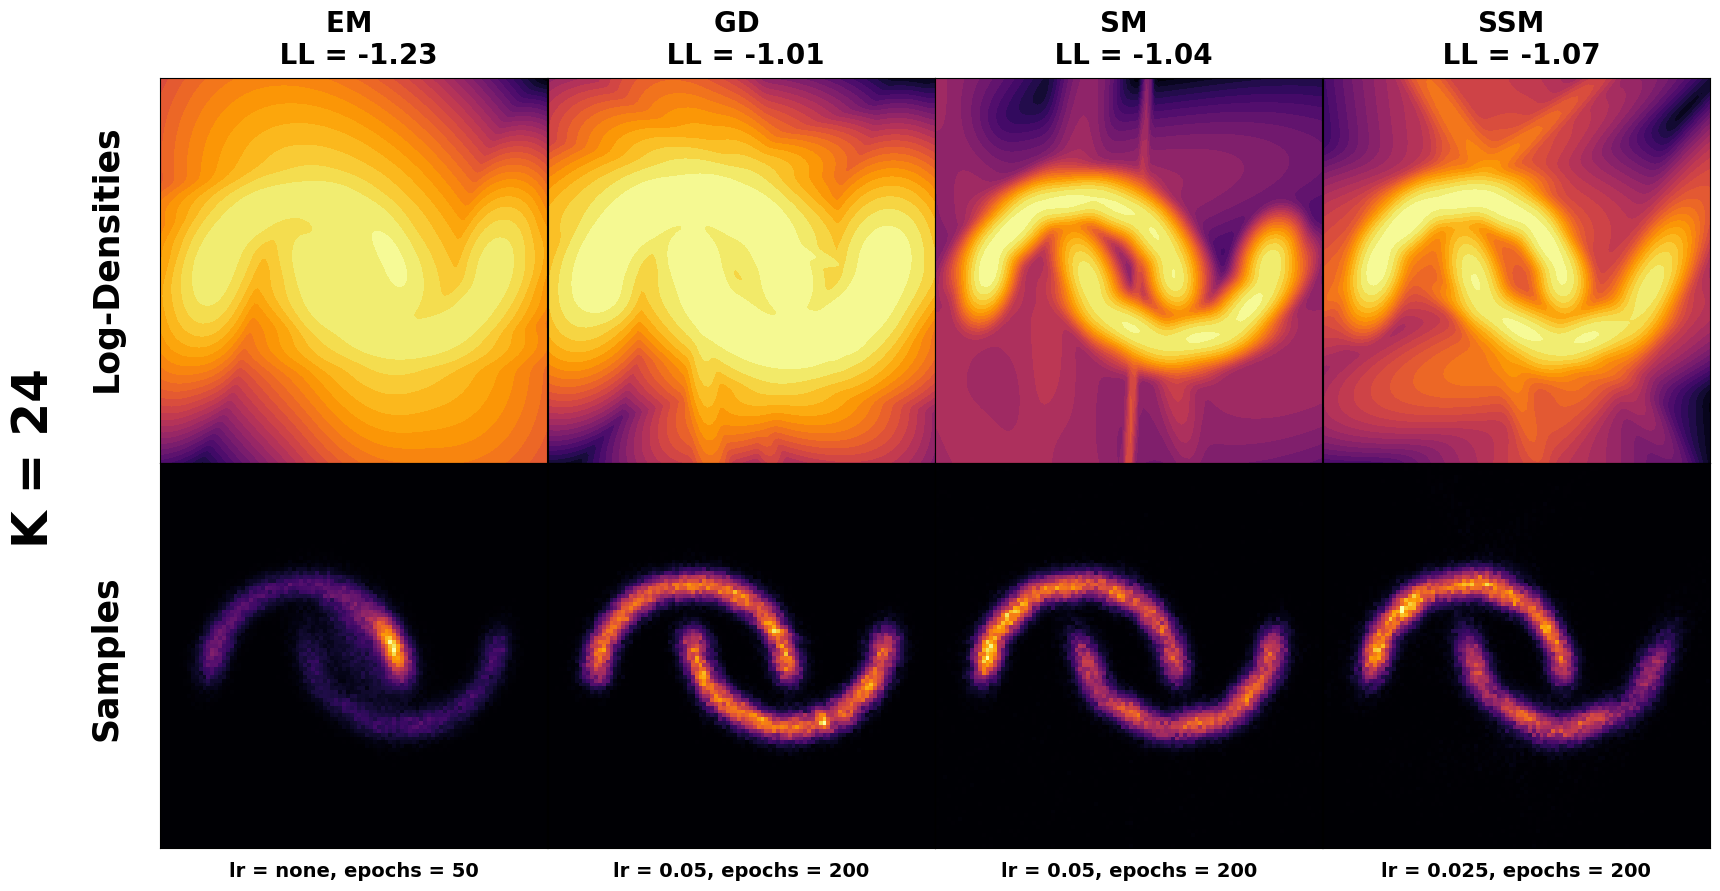
\includegraphics[width=0.9\textwidth]{figures/halfmoons/halfmoons_24.png}}
    \caption{Densities and Samples for the halfmoon dataset}
    \label{fig:exp_moons}
\end{figure}
\newpage
\begin{figure}[H]
    \centering
    \makebox[\textwidth][c]{\hspace*{-1cm} 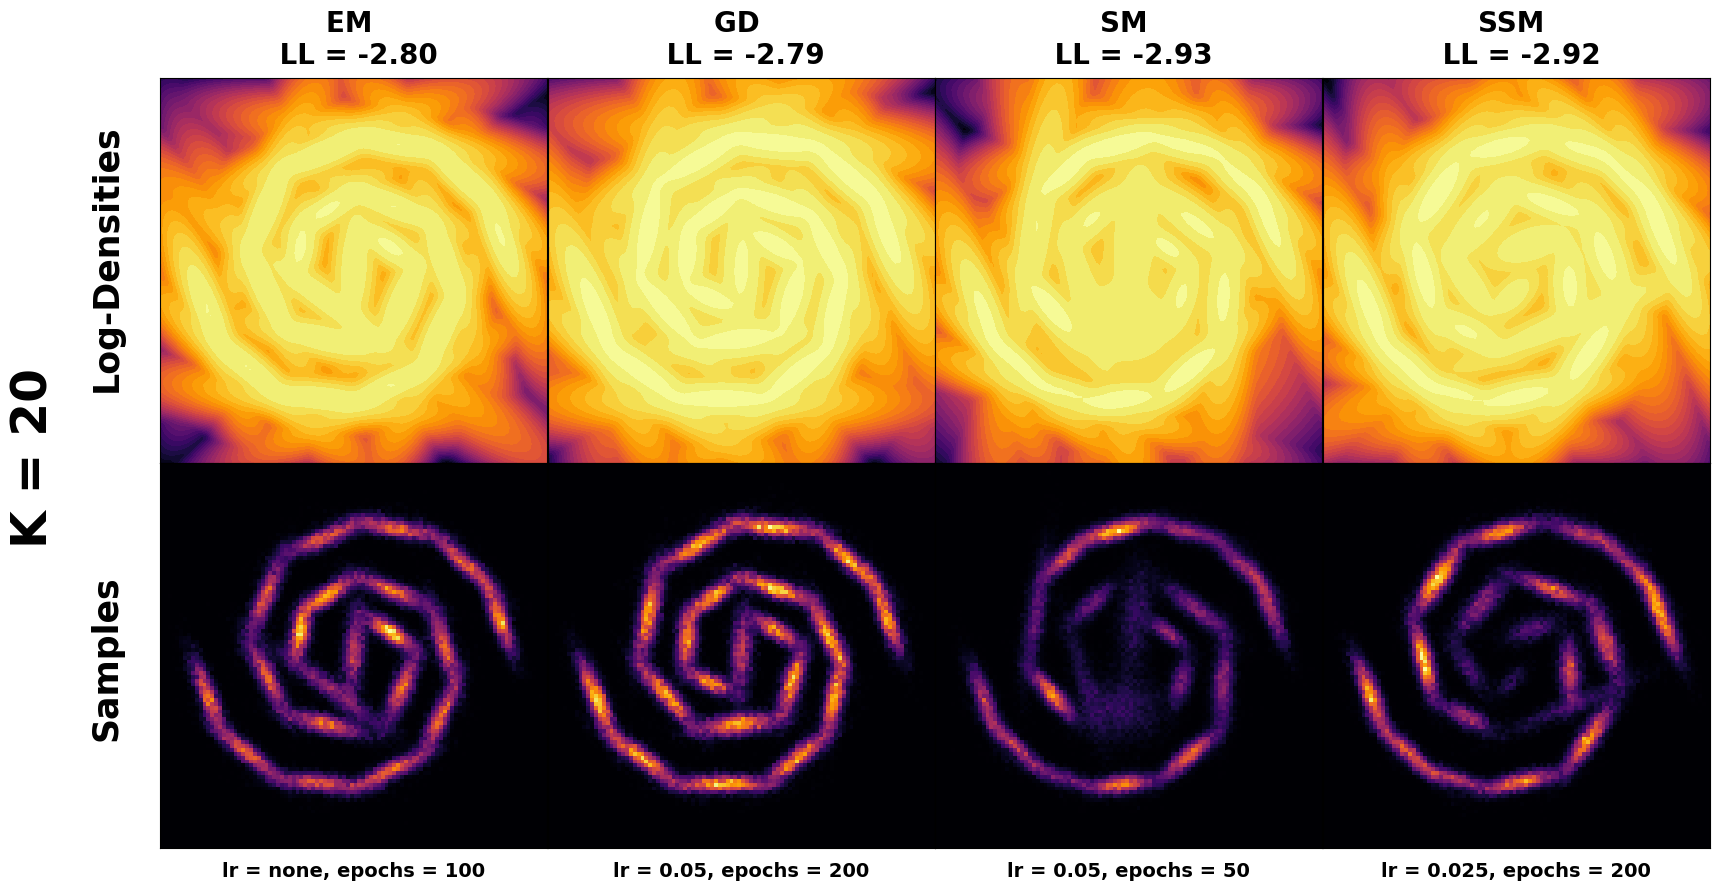
\includegraphics[width=0.9\textwidth]{figures/spirals/spirals_20.png}}
    \vskip 5pt
    \makebox[\textwidth][c]{\hspace*{-1cm} 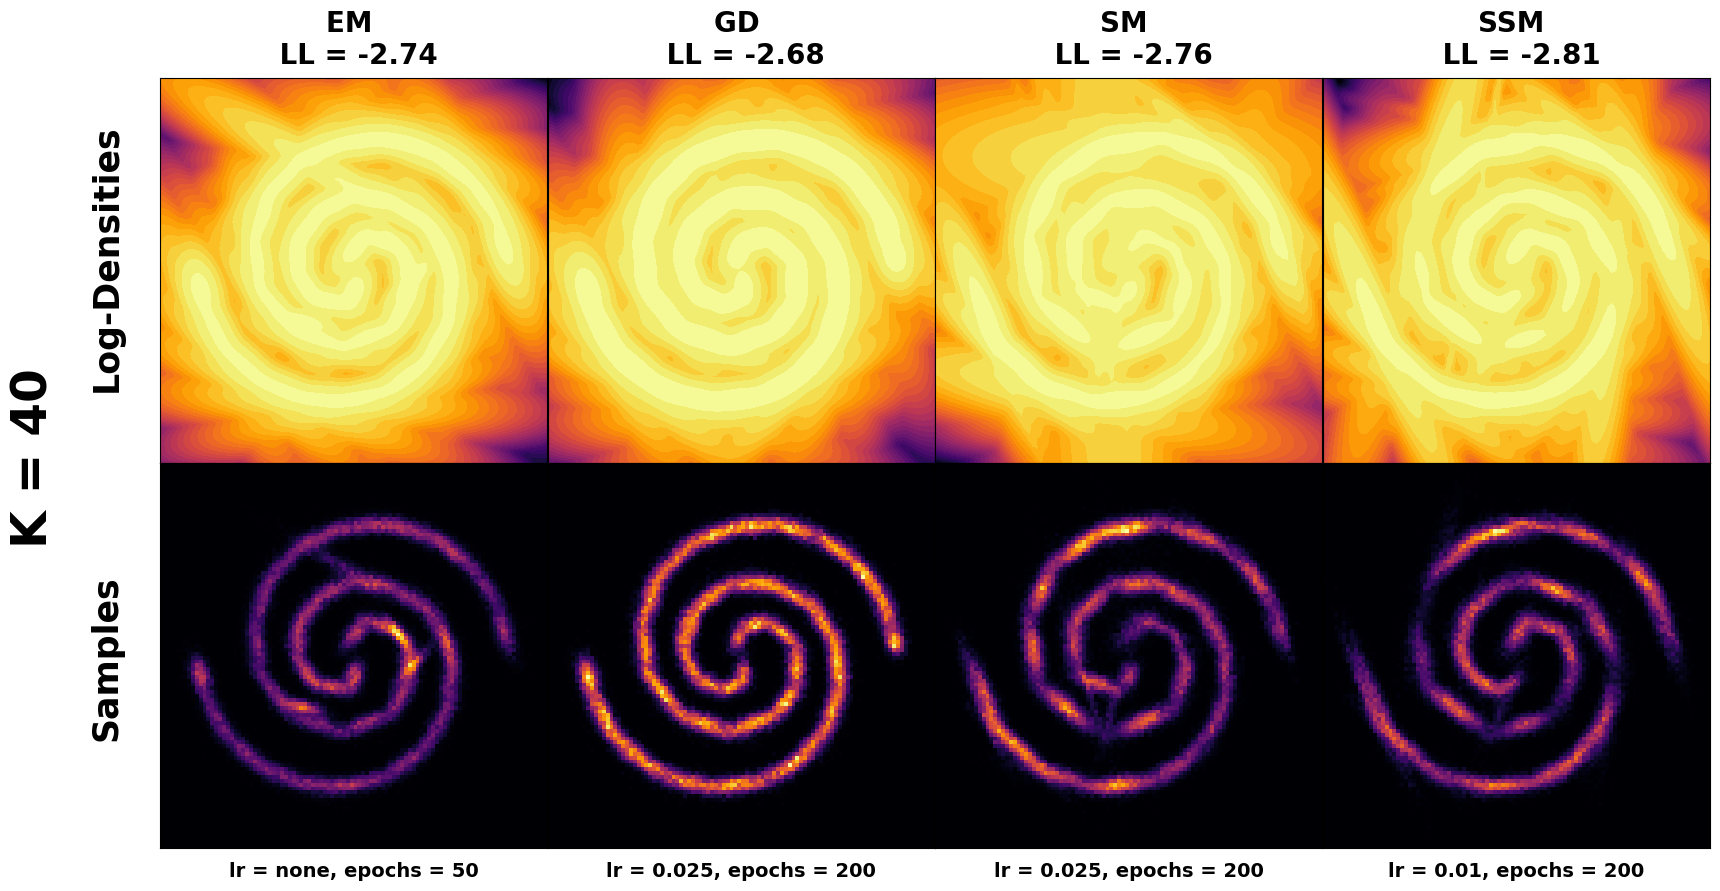
\includegraphics[width=0.9\textwidth]{figures/spirals/spirals_40.png}}
    \vskip 5pt
    \makebox[\textwidth][c]{\hspace*{-1cm} 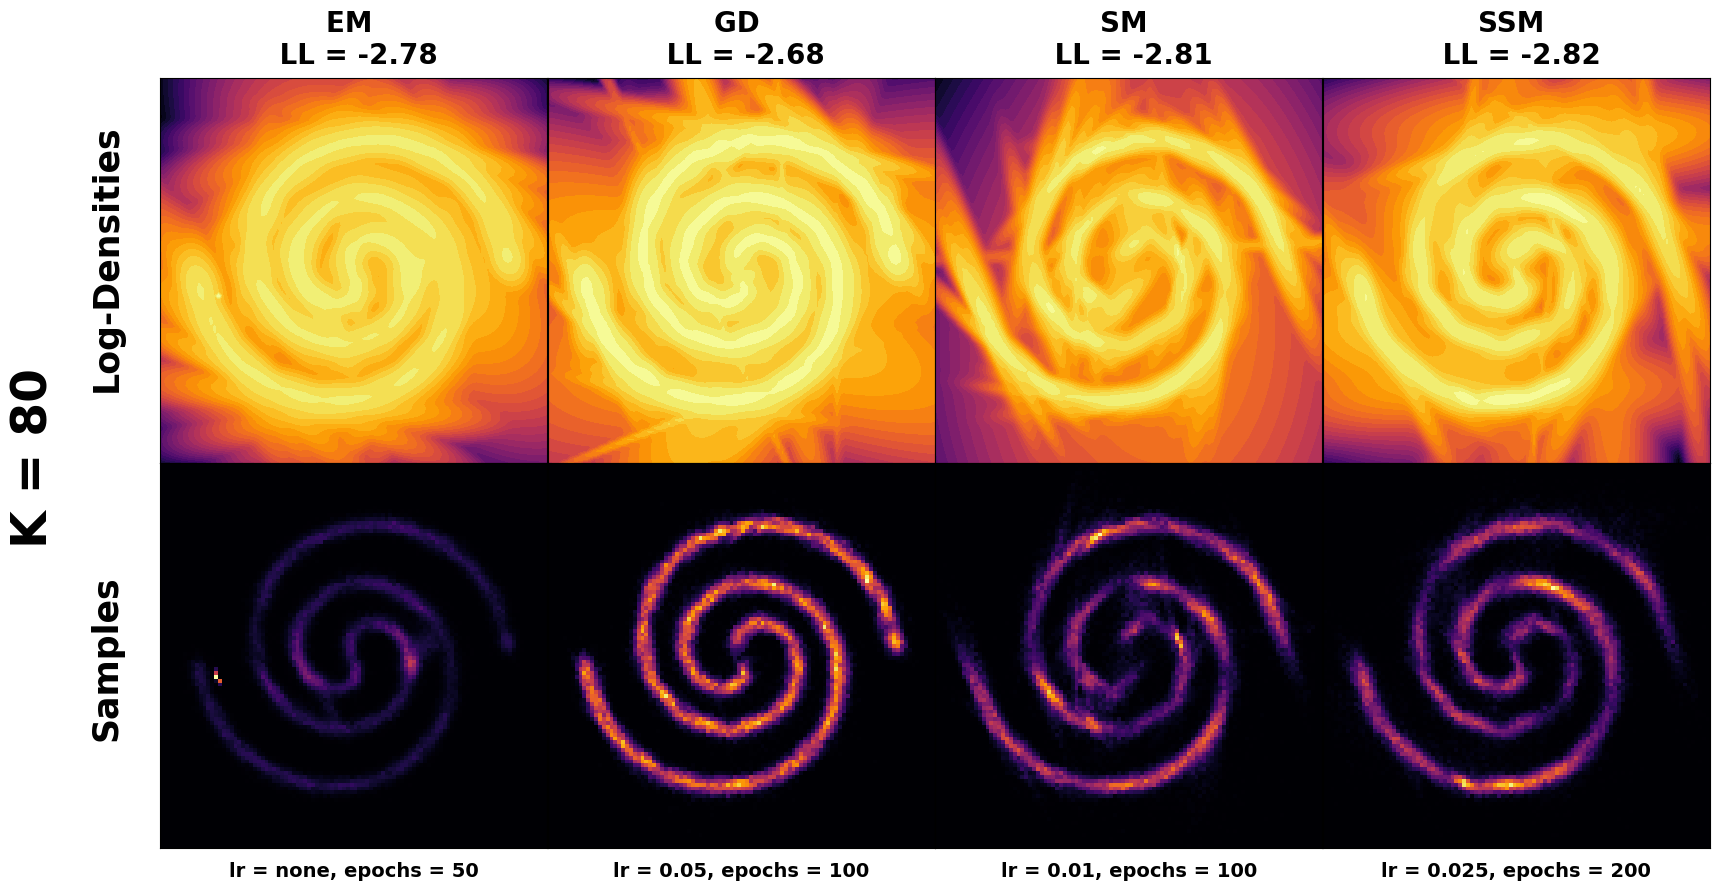
\includegraphics[width=0.9\textwidth]{figures/spirals/spirals_80.png}}
    \caption{Densities and Samples for the spirals dataset}
    \label{fig:exp_moons}
\end{figure}
\newpage
\begin{figure}[H]
    \centering
    \makebox[\textwidth][c]{\hspace*{-1cm} 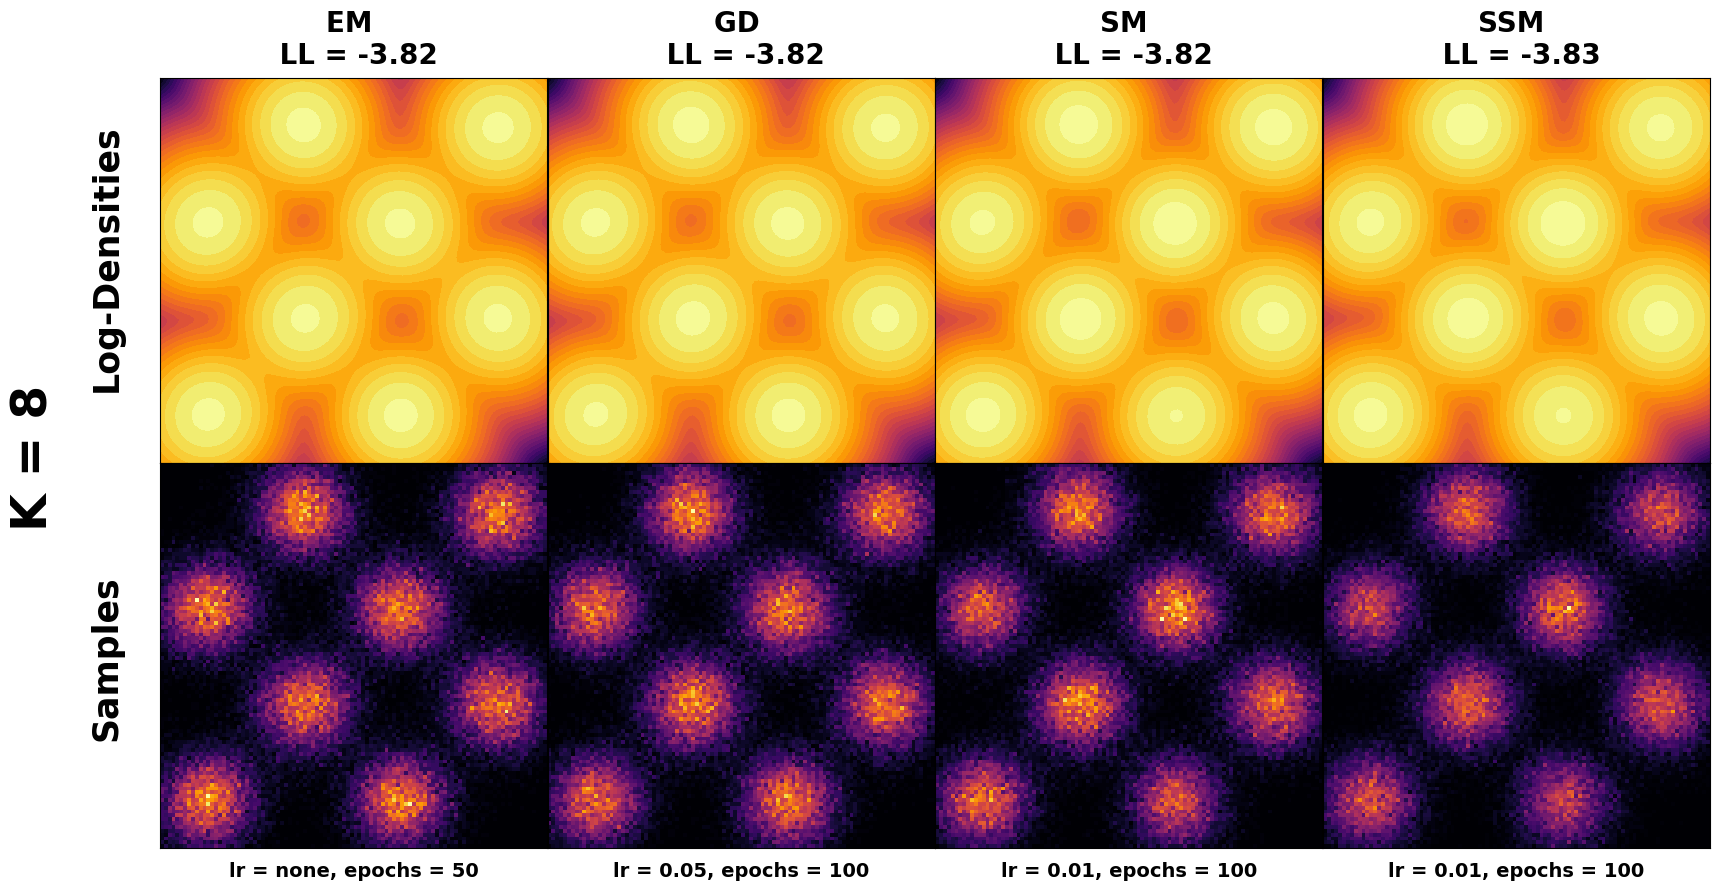
\includegraphics[width=0.9\textwidth]{figures/board_8.png}}
    \vskip 5pt
    \makebox[\textwidth][c]{\hspace*{-1cm} 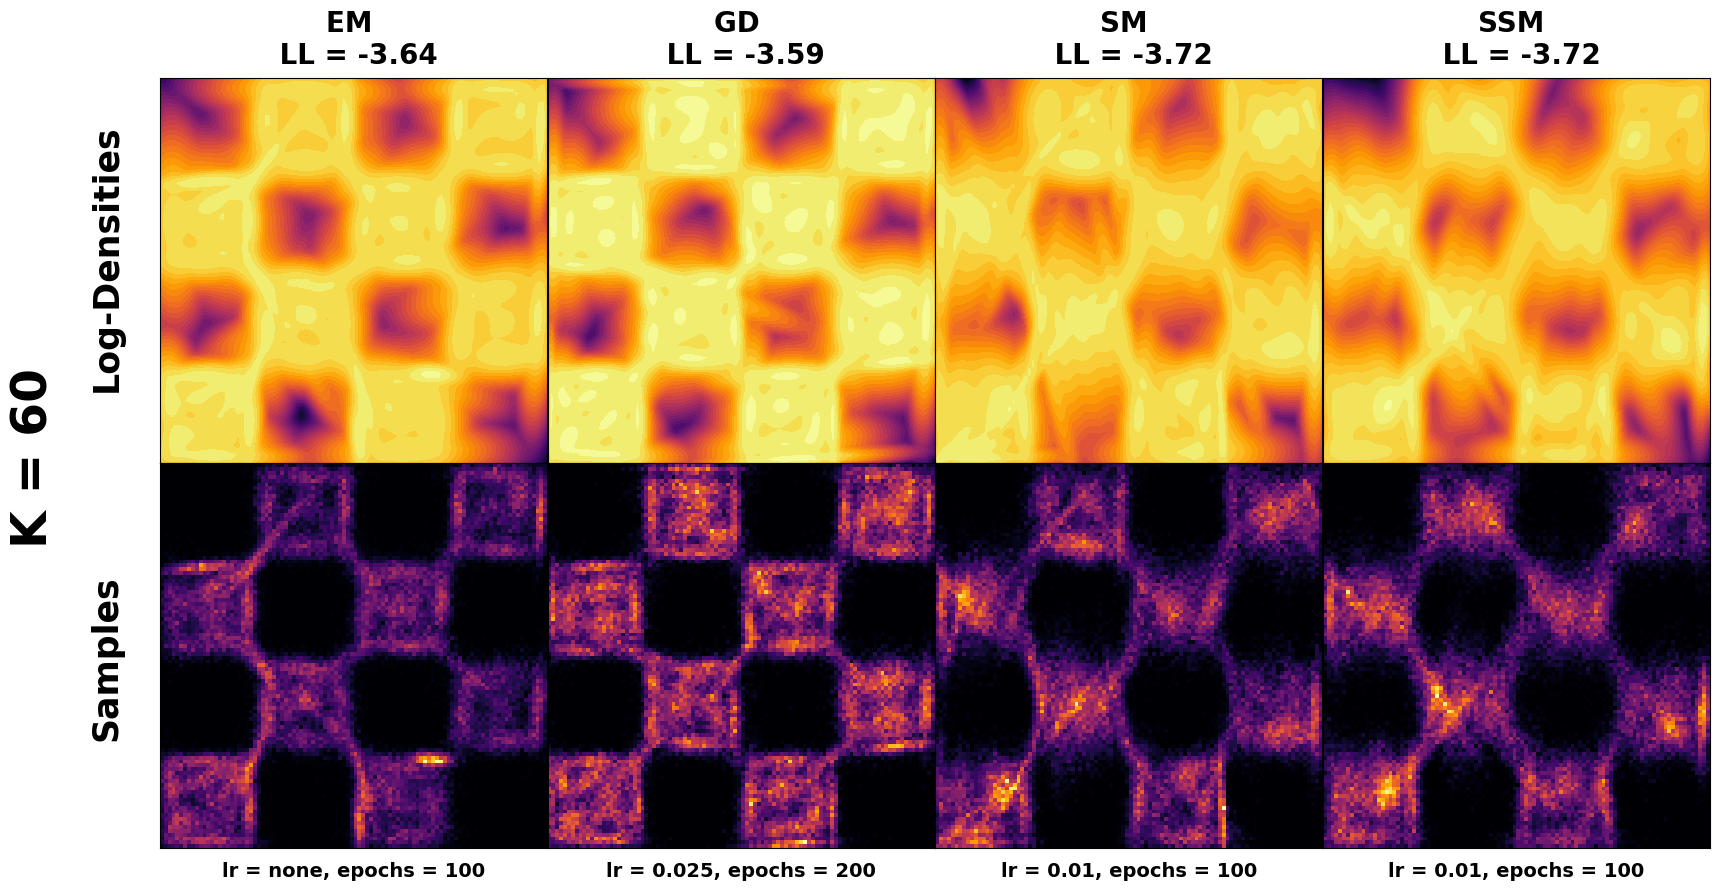
\includegraphics[width=0.9\textwidth]{figures/board_60.png}}
    \vskip 5pt
    \makebox[\textwidth][c]{\hspace*{-1cm} 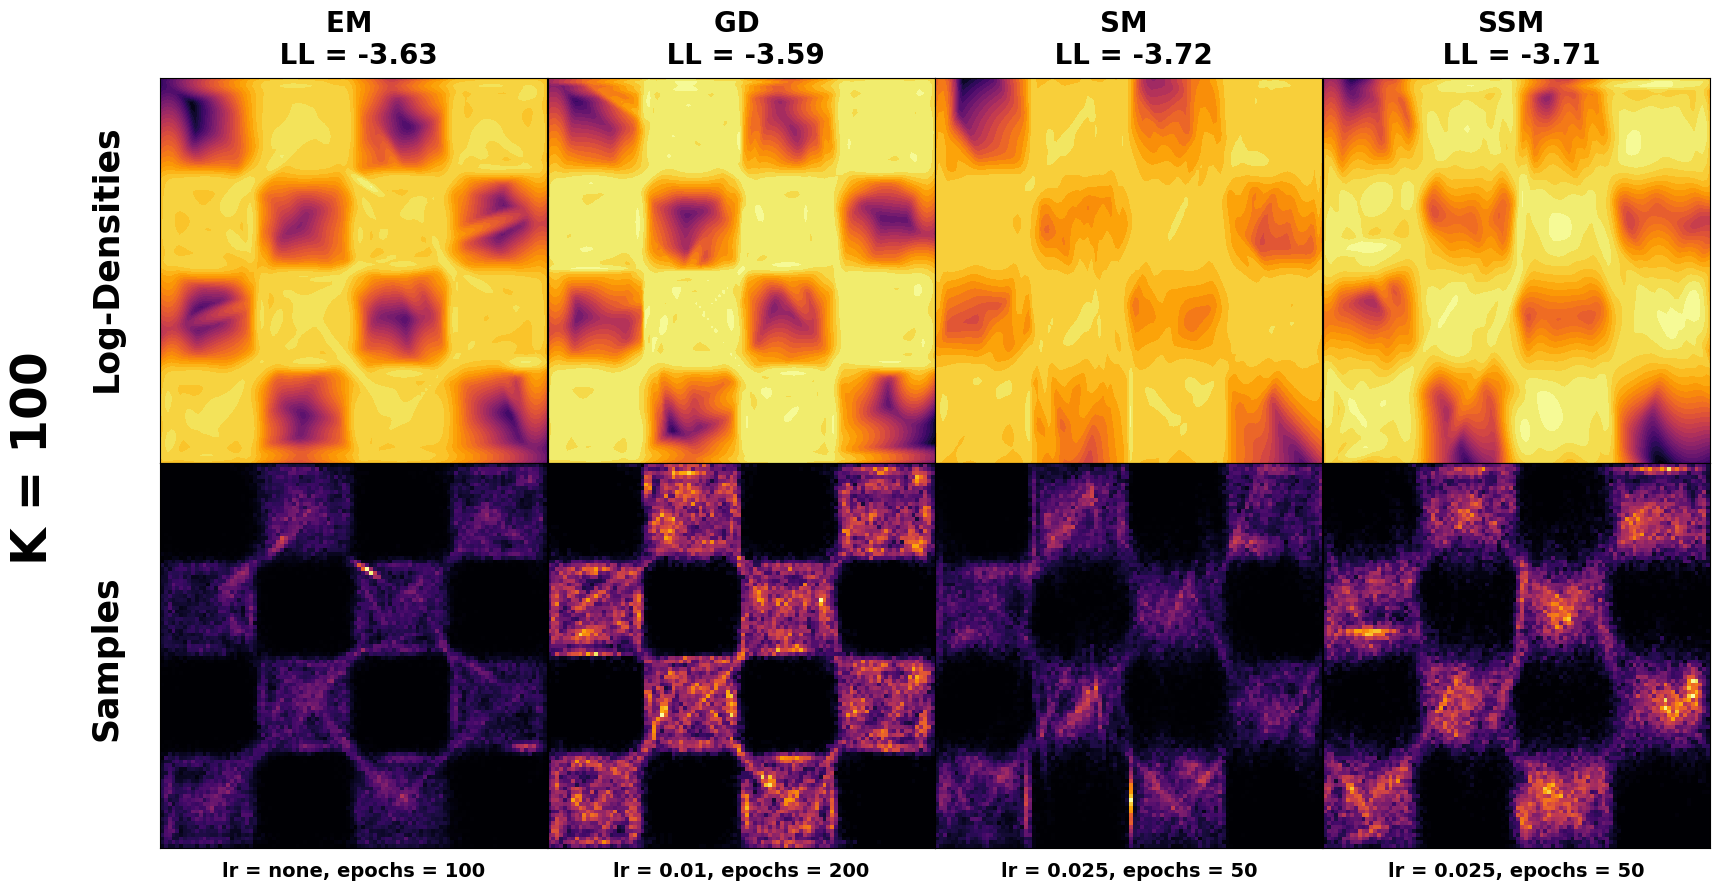
\includegraphics[width=0.9\textwidth]{figures/board_100.png}}
    \caption{Densities and Samples for the board dataset}
    \label{fig:exp_moons}
\end{figure}
\newpage

\subsection{Performance Analysis}
\label{sec:2d_exp2}

To gain further insight in how the learning process differs for each algorithm we chose a dataset and a set of hyperparameters
where all algorithms perform somewhat similar and analyzed the Negative Log-Likelihood (NLL) over Training Iterations. 
Estimated density and samples and now also the mentioned training curve can be seen in Figure \ref{fig:halfmoons_10_logp}.

Note that because all algorithms except Sliced Score Matching are deterministic, we did multiple runs ($10$) for SSM and plotted the mean value 
with the standard deviation shaded. 

\begin{figure}[H]
    \centering
    \makebox[\textwidth][c]{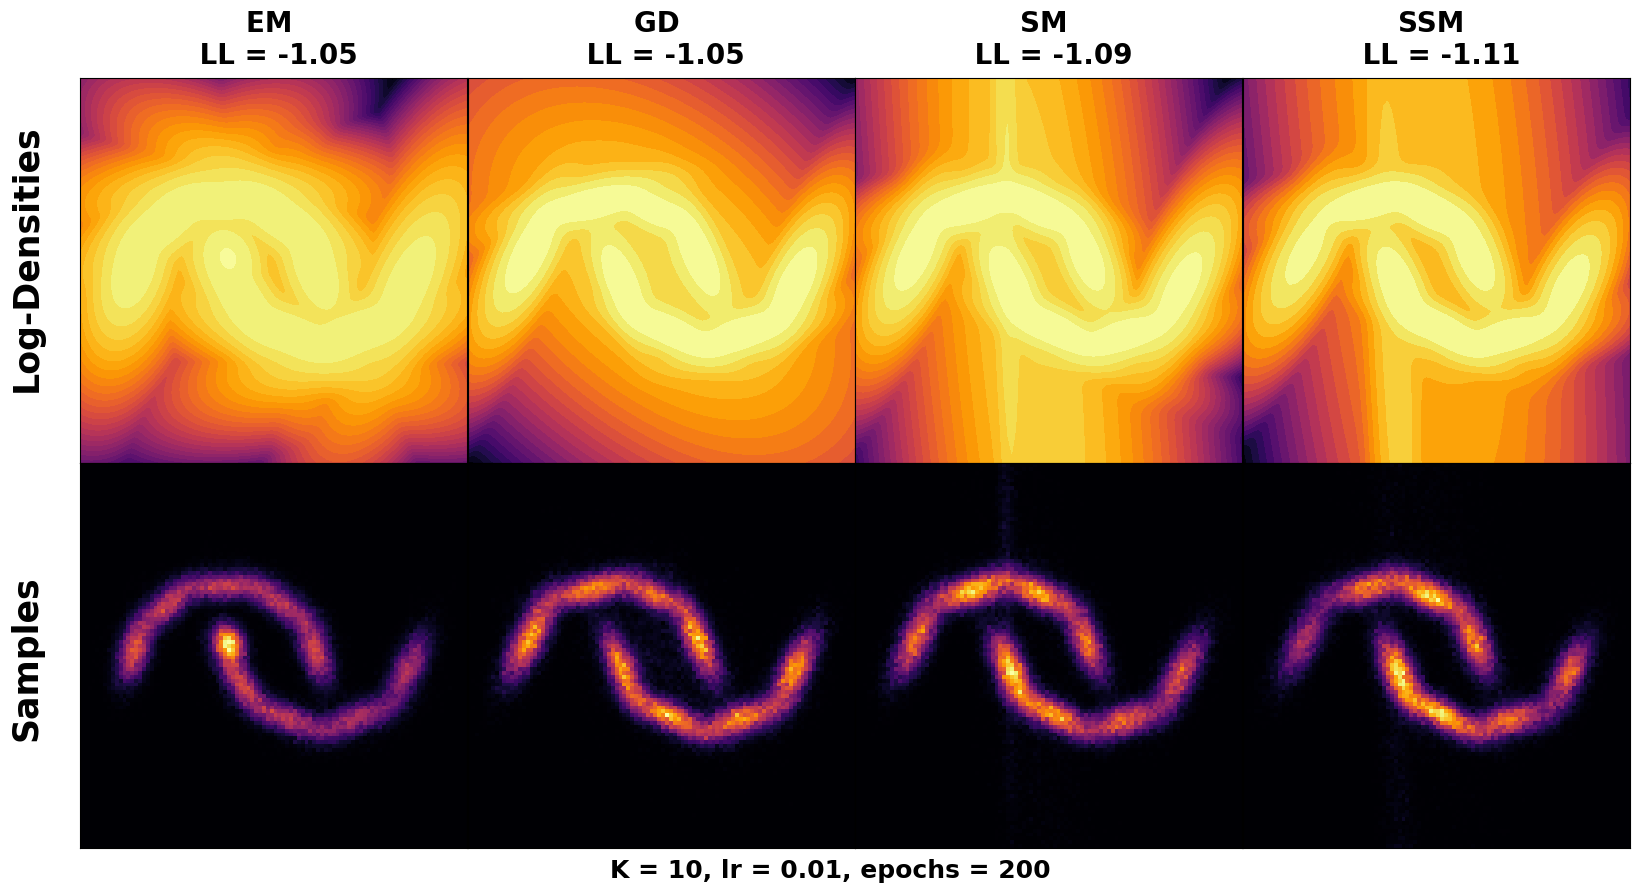
\includegraphics[width=0.8\textwidth]{figures/halfmoons/10_kmeans.png}}
    \makebox[\textwidth][c]{\hspace{-0.4cm} 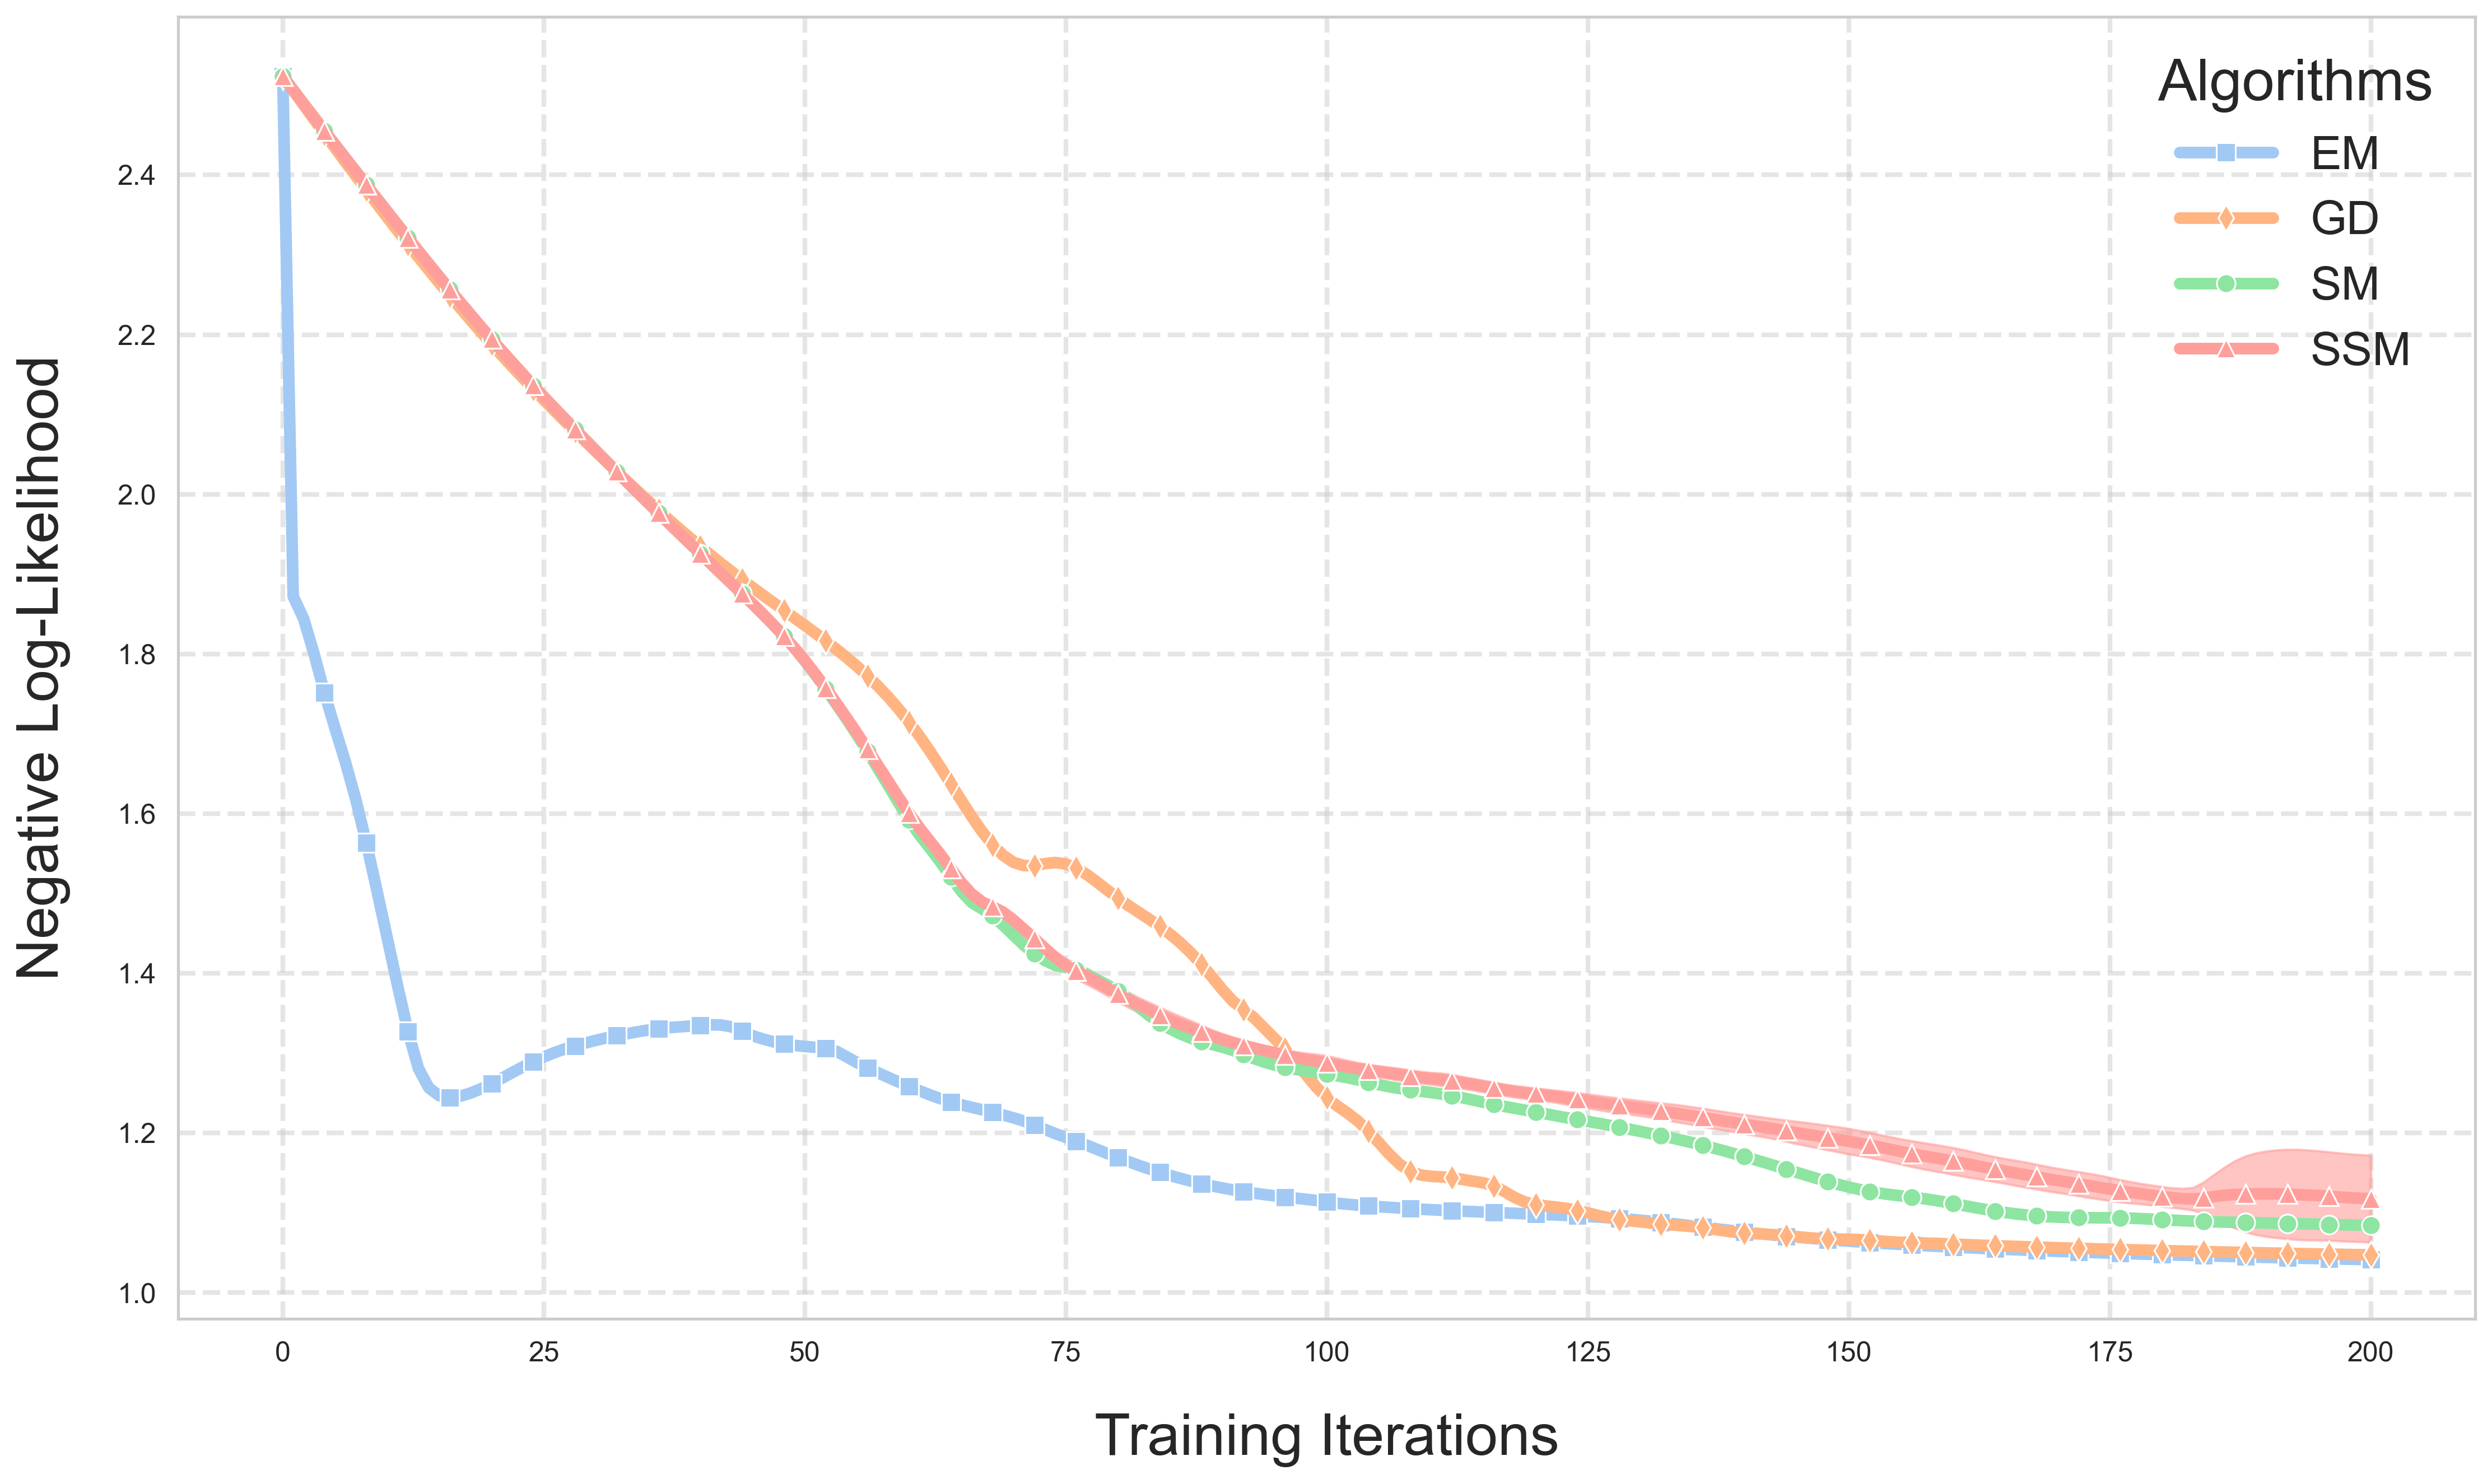
\includegraphics[width=0.9\textwidth]{figures/halfmoons/10_kmeans_logp.png}}
    \caption{Densities, Samples and NLL over Training Iterations}
    \label{fig:halfmoons_10_logp}
\end{figure}

First, we see that on average SSM performs somewhere in the ballpark of SM but usually a little worse, which 
makes sense since SSM is only an approximation of SM. Sometimes the stochastic nature of SSM can also 
by sheer luck yield better results. Note that when increasing the number of slices, which were $1$ for all 
experiments up until now, we saw that SSM increasingly gives a better approximation of SM.

Another clearly noticeable result is that EM appears to learn the fastest and all the gradient-based algorithms
behave quite similarly. This was reproducible for all other datasets and hyperparameter configurations as well. 
However note that in the Figures above, we are only looking at NLL over Epochs, so we are not accounting for the 
duration of a single epoch, but this matters a lot in practice.
When running all algorithms for a specific amount of time, the differences increase considerably. 

\begin{figure}[H]
    \centering
    \makebox[\textwidth][c]{\hspace{-0.4cm} 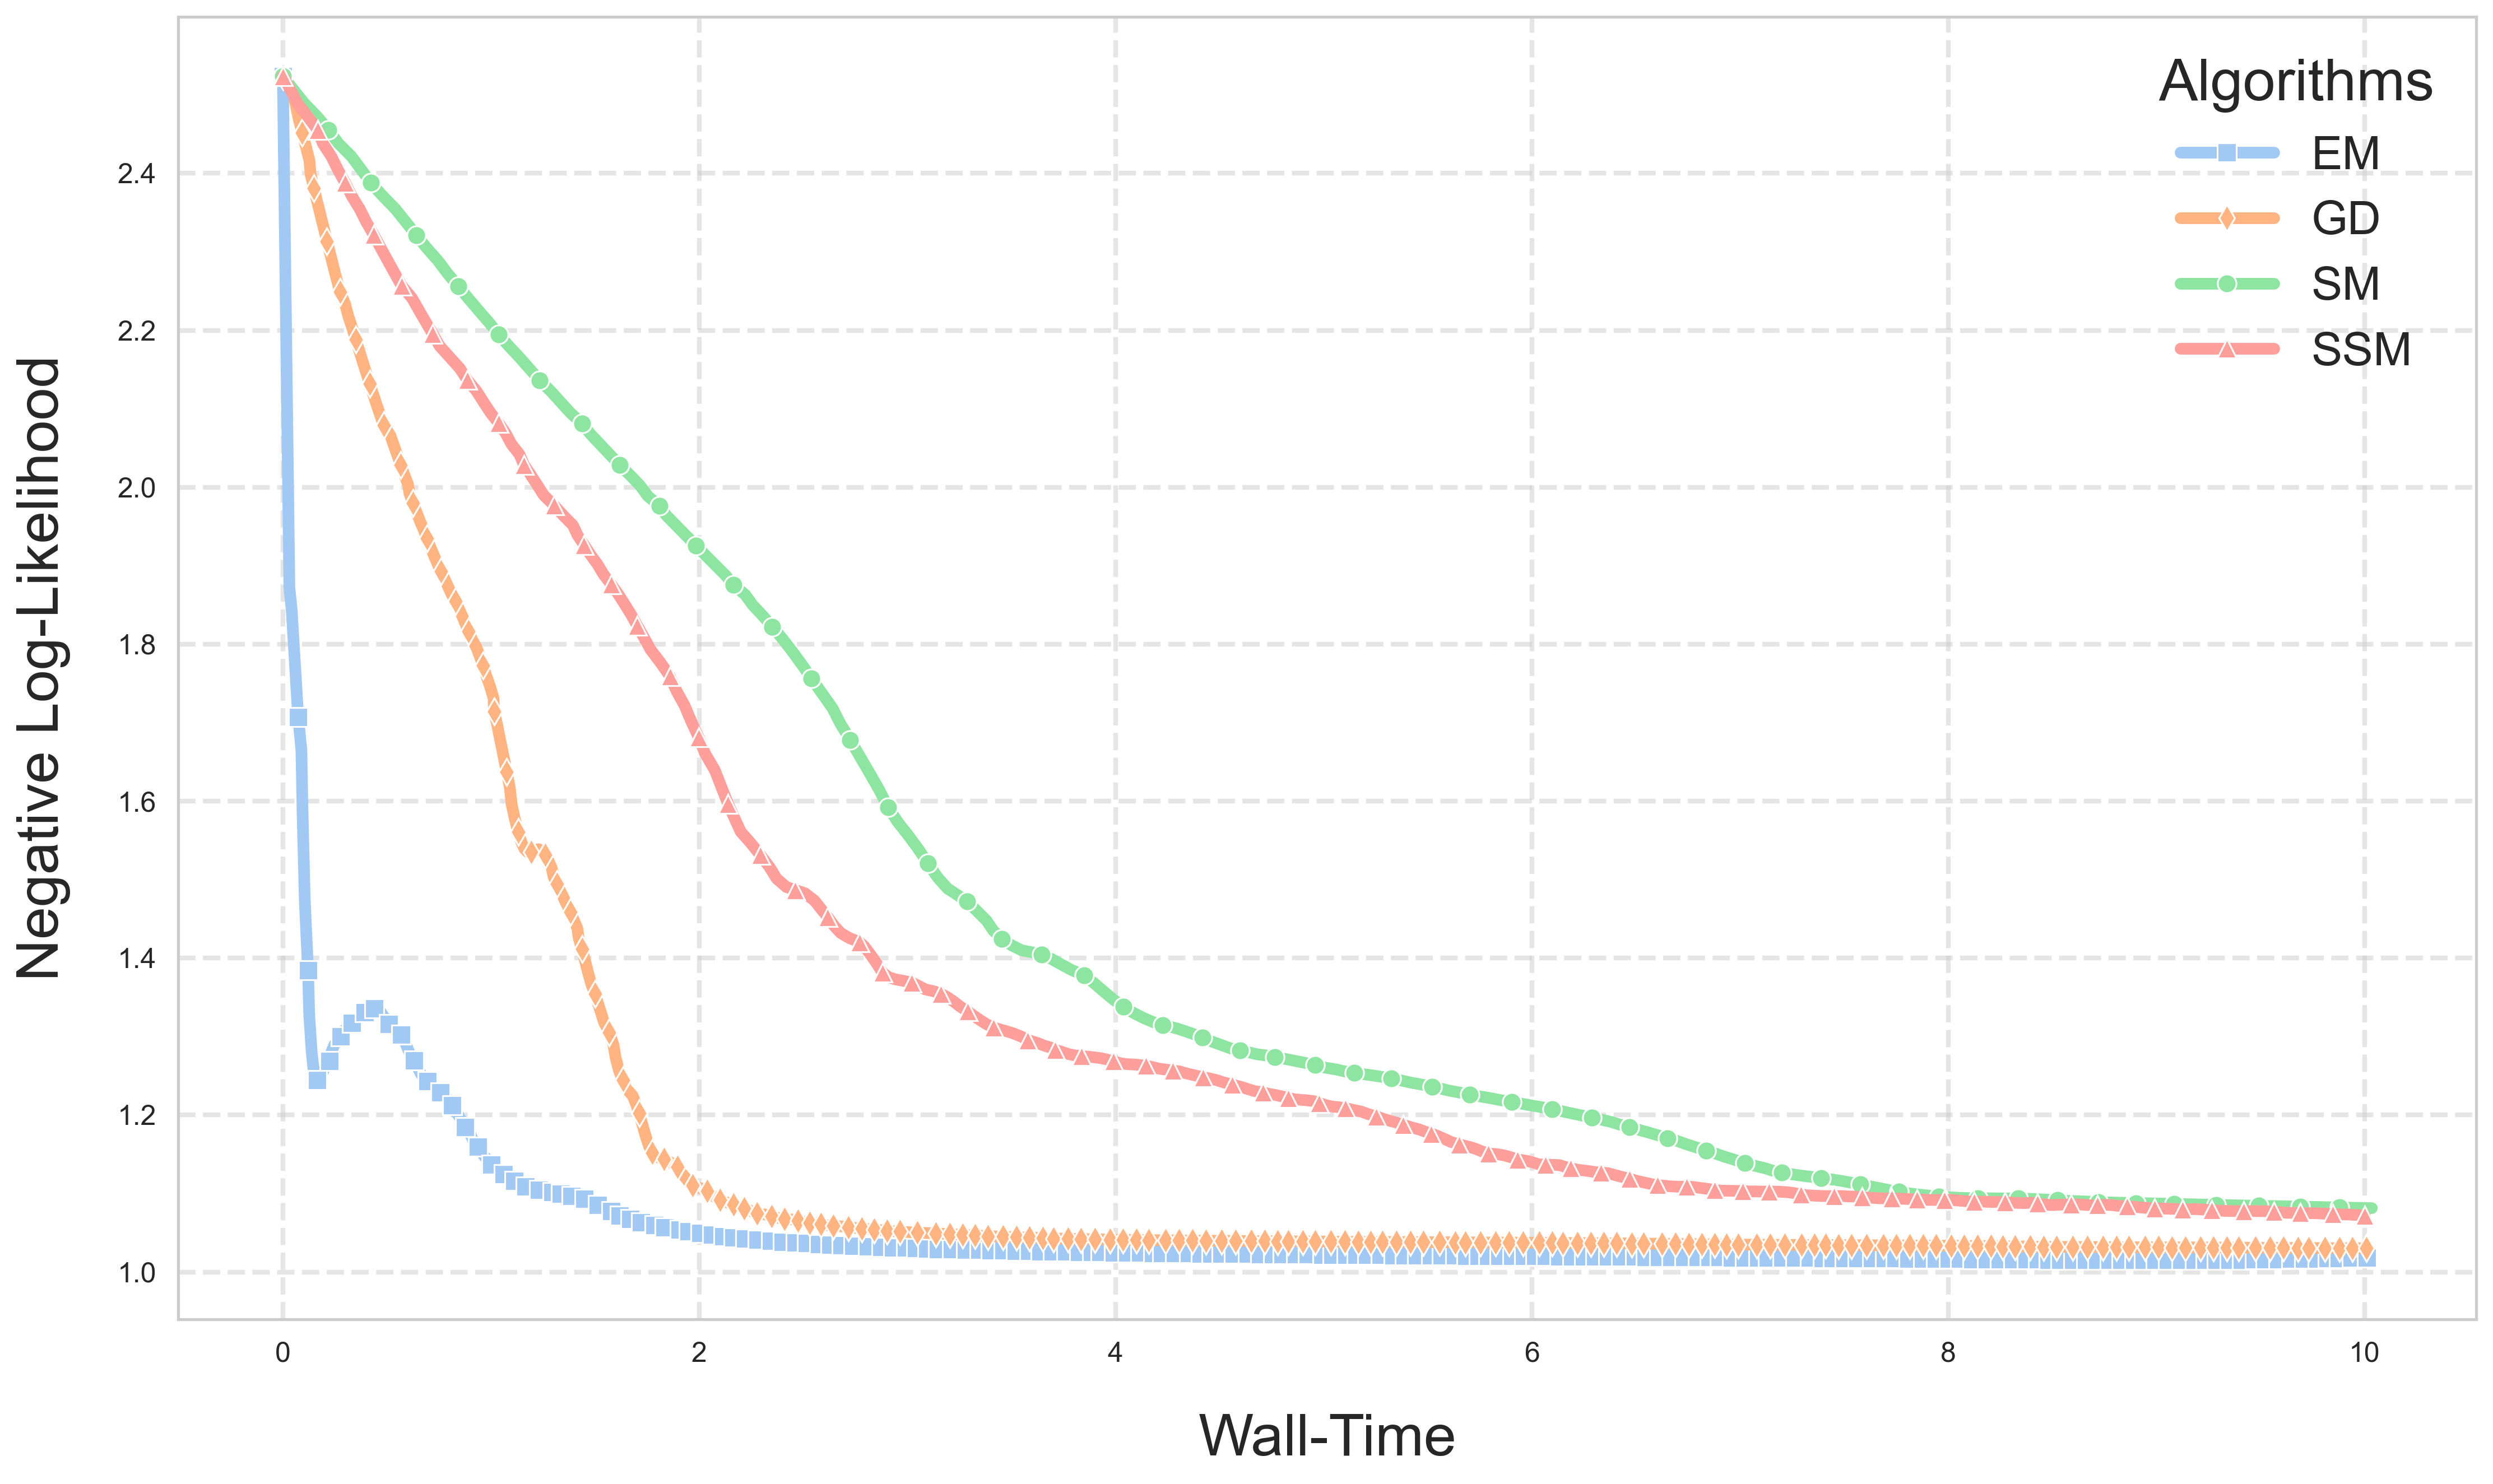
\includegraphics[width=0.9\textwidth]{figures/halfmoons/wall_time.png}}
    \caption{NLL over Time}
    \label{fig:spirals_30_kmeans}
\end{figure}

EM and GD appear considerably faster than their Score Matching alternatives, in fact while GD on average only takes 
around $1.1$ times as long as EM, SSM takes around twice as long and SM around $2.5$ times as long.

\subsection{Random Initialization}
\label{sec:2d_exp3}

\begin{figure}[H]
    \centering
    \begin{subfigure}[b]{0.49\textwidth} 
        \centering
        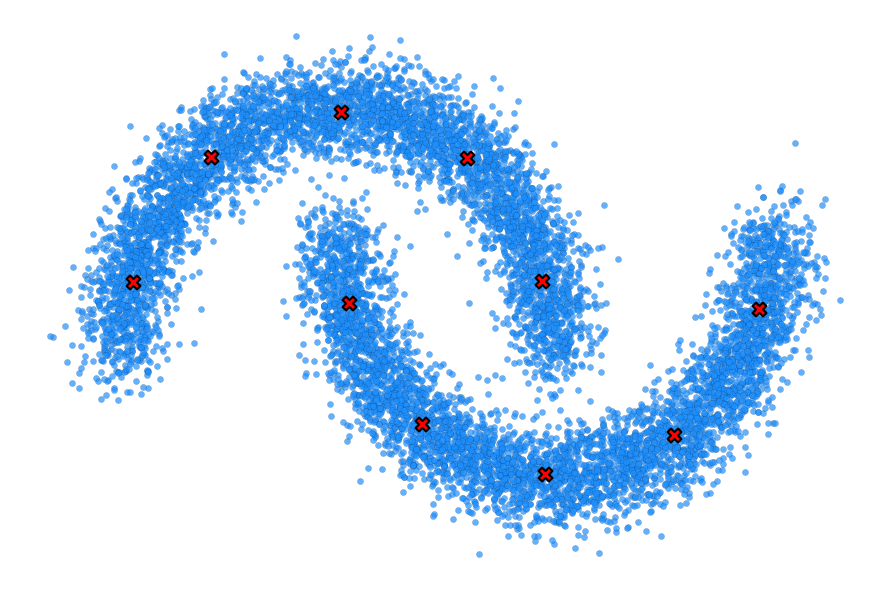
\includegraphics[width=\textwidth]{figures/halfmoons/10_kmeans_data.png}
        \caption{KMeans}
    \end{subfigure}
    \begin{subfigure}[b]{0.49\textwidth} 
        \centering
        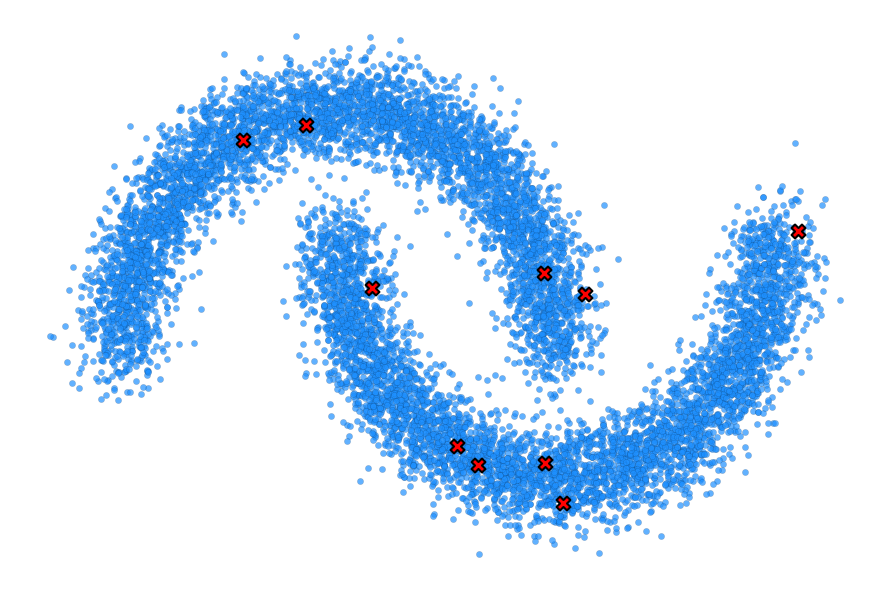
\includegraphics[width=\textwidth]{figures/halfmoons/10_random1_data.png} 
        \caption{Random}
    \end{subfigure} 
    \caption{KMeans vs. Random Initialization of means}
    \label{fig:kmeans_vs_rand}
\end{figure}

Another point we wanted to examine was the initialization of the learnable parameters. 

With our data it is quite straightforward to initialize the means, which up to now has been done with KMeans, but this is not always the case.
Also initializing the weights uniformly conveniently makes a lot of sense with our data, however the initialization of both of these 
learnable parameters can be problematic and a lot of times this has to be done randomly. \\
Therefore we also analyzed how each algorithm 
behaves when these parameters are initialized randomly. 

To initialize the means we draw $K$ random data points from our training data and 
to initialize the weights we just draw random numbers from $0$ to $1$ and normalize them so they sum to one.

In Figure \ref{fig:halfmoons_10_random_logp} the mean Log-Likelihood and standard deviation over $10$ runs with random initialization in each run can be seen. 

\begin{figure}[H]
    \centering
    \makebox[\textwidth][c]{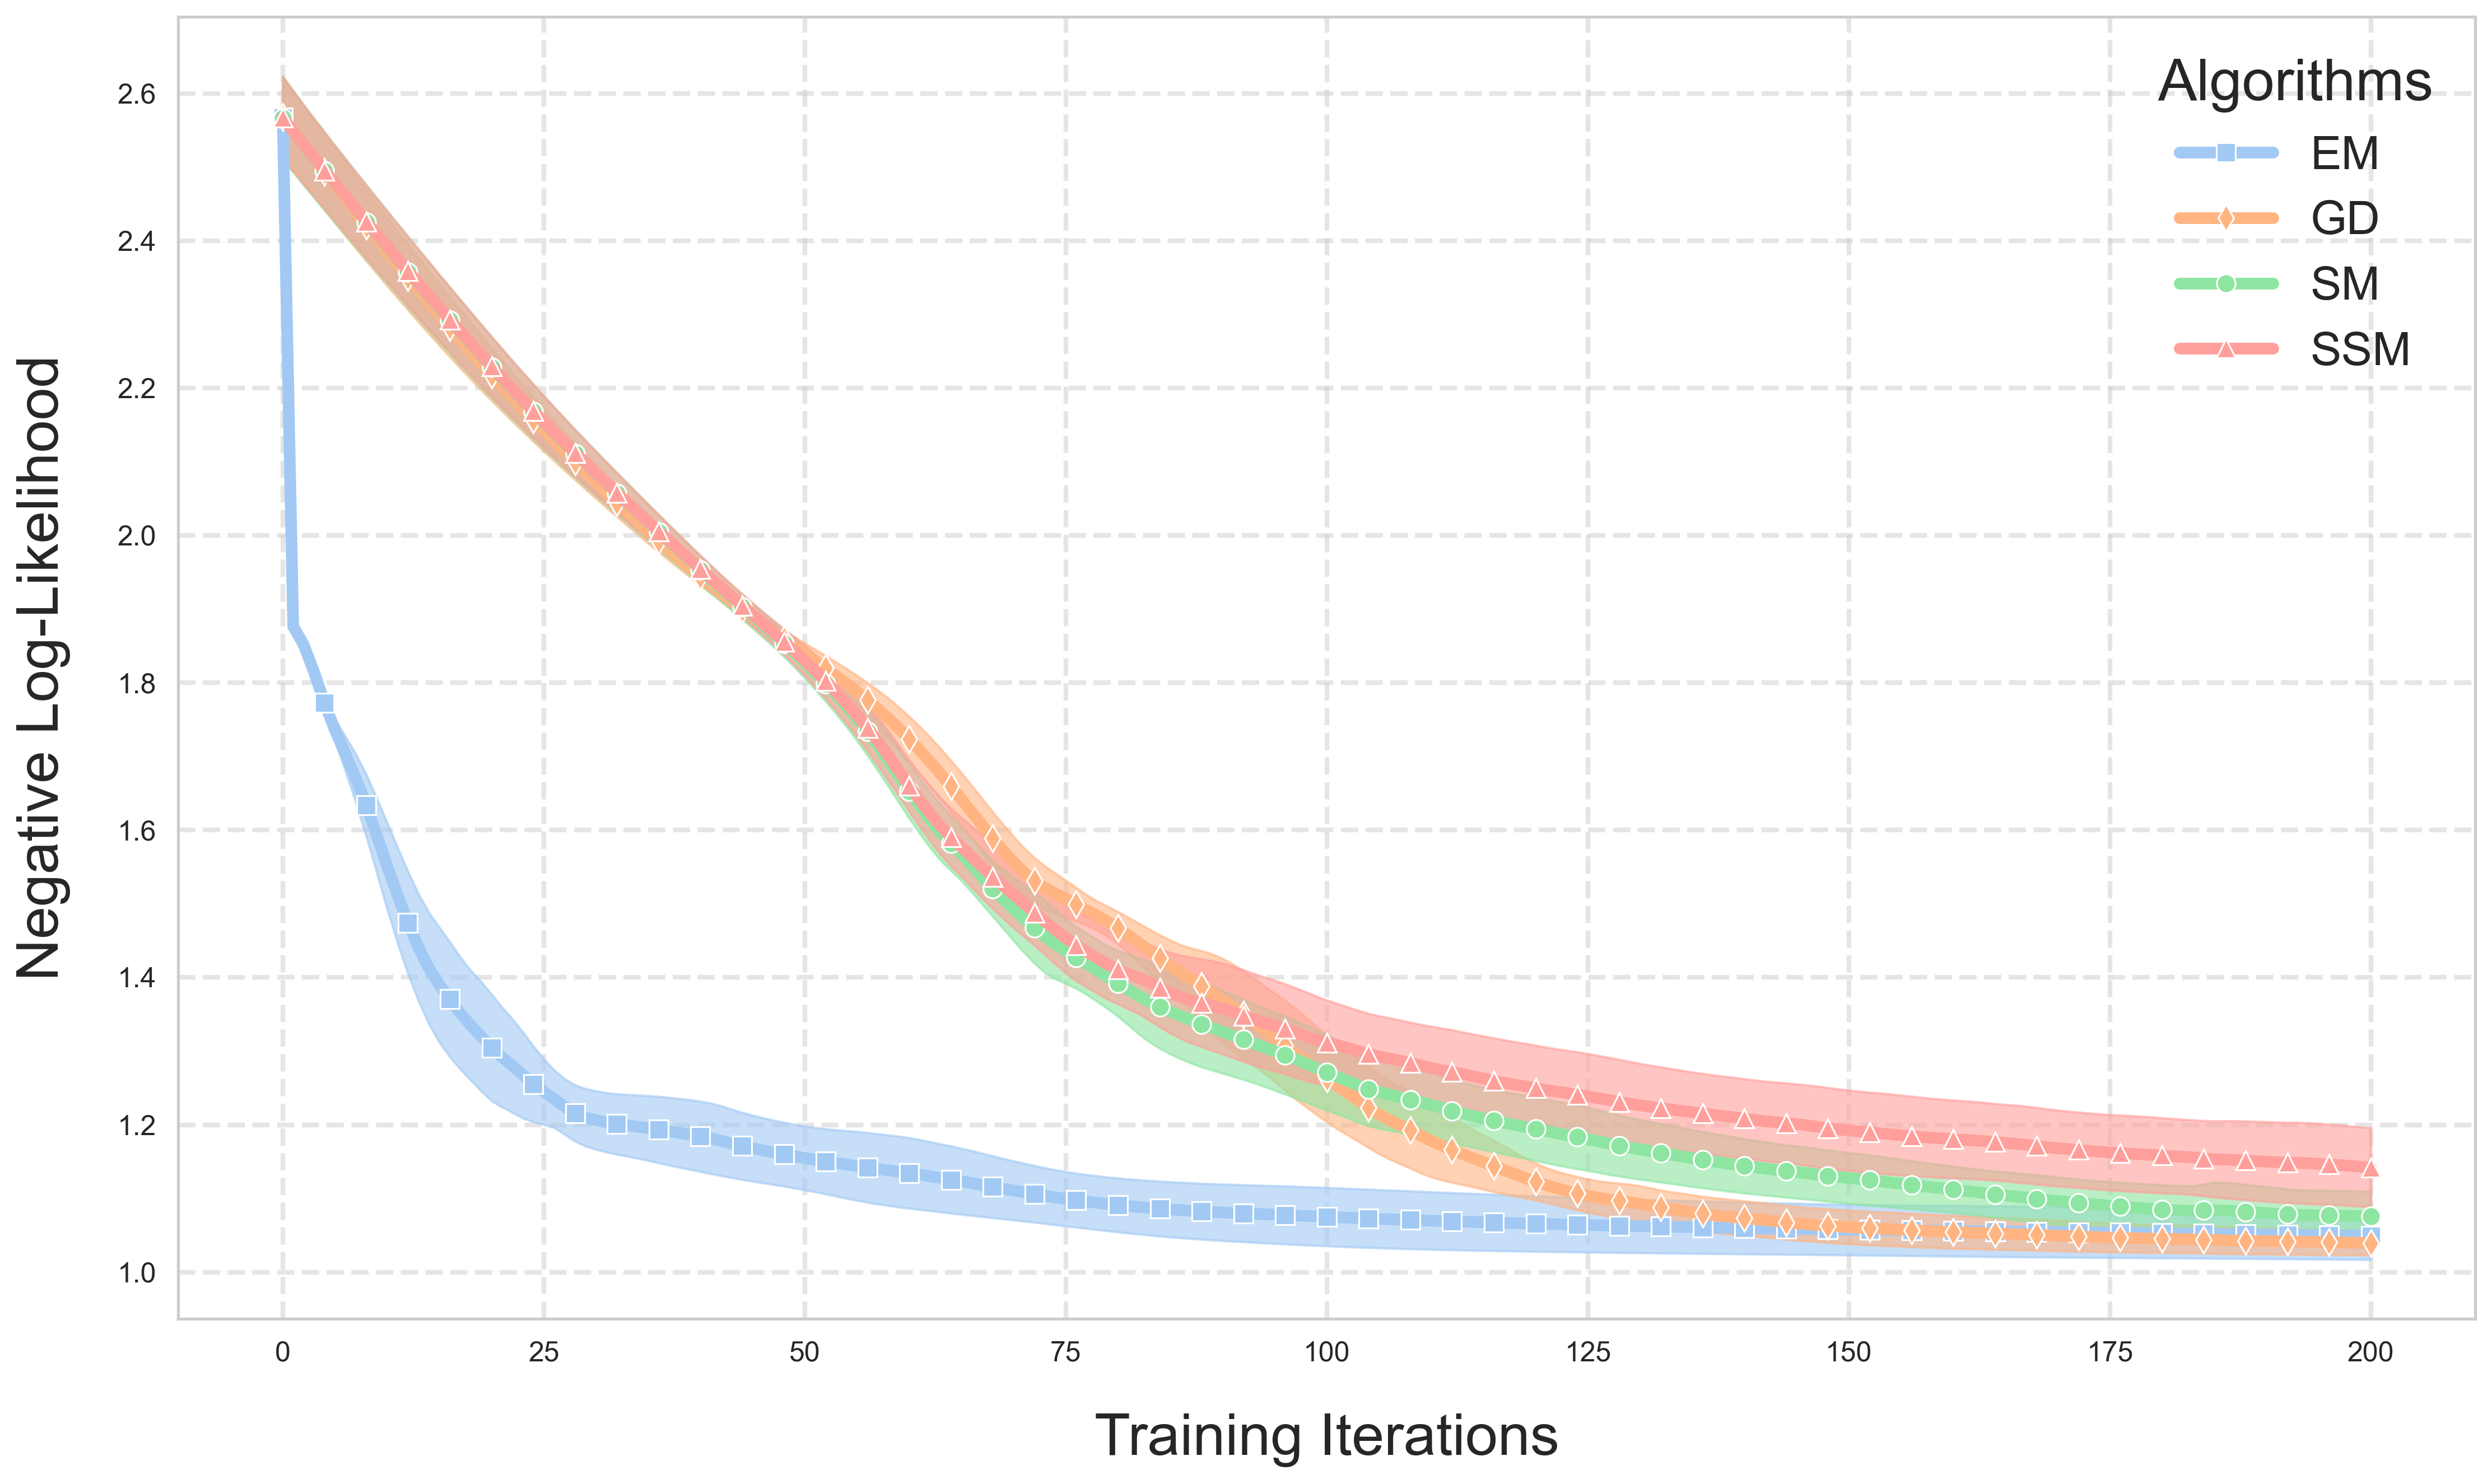
\includegraphics[width=0.9\textwidth]{figures/halfmoons/10_random_logp.png}}
    \caption{Negative Log Likelihood over Epochs with random parameter initialization}
    \label{fig:halfmoons_10_random_logp}
\end{figure}

On this simple dataset it appears that random initialization performs relatively similar to the KMeans initialization when comparing 
to the NLL over Epochs curve from Figure \ref{fig:halfmoons_10_logp}. For some concrete results (Densities and Samples) refer to the Appendix \ref{sec:app_halfmoons_rand}.

We repeated Experiments \ref{sec:2d_exp2} and \ref{sec:2d_exp3} for the spirals dataset, results can be found in the Appendix \ref{sec:app_spirals}.

\section{Images Density Estimation}

To train an EinsumNetwork with our target algorithms, we used the provided demo which uses either the MNIST of FashionMNIST Dataset \cite{mnist} and integrated 
our algorithms. Note that we left out Score Matching since training already took very long and we were limited with our compute power. 

We left the model related hyperparameters as they were provided in the framework and only tuned the training specific hyperparameters 
(iterations and learning rate) to produce the best possible results for each algorithm. 
On a side note, this setup resulted in $204146$ learnable parameters for the EinsumNetwork, for comparison the most 
complex 2D model we used with $100$ mixture components had $700$ learnable parameters. 

Samples and Test Log-Likelihood for three different classes of both MNIST and FashionMNIST can be seen below. \\
Note that these can't really be reproduced since the demo uses mini-batch learning which introduces stochasticity. 

\begin{figure}[H]
    \centering
    \begin{subfigure}[b]{0.24\textwidth}
        \centering
        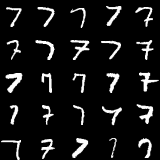
\includegraphics[width=\textwidth]{figures/einsum/7mnist_ground_truth.png}
        \caption{Ground Truth}
    \end{subfigure}
    \begin{subfigure}[b]{0.24\textwidth}
        \centering
        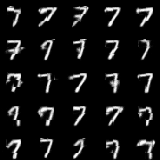
\includegraphics[width=\textwidth]{figures/einsum/7mnist_EM.png}
        \caption{EM (LL: -11570)}
    \end{subfigure}
    \begin{subfigure}[b]{0.24\textwidth}
        \centering
        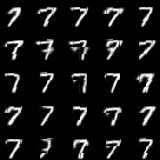
\includegraphics[width=\textwidth]{figures/einsum/7mnist_SGD.png} 
        \caption{SGD (LL: -12925)}
    \end{subfigure}
    \begin{subfigure}[b]{0.24\textwidth}
        \centering
        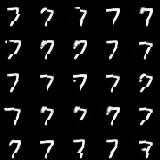
\includegraphics[width=\textwidth]{figures/einsum/7mnist_SSM.png}
        \caption{SSM (LL: -16447)}
    \end{subfigure}
    \caption{Samples and Log-Likelihood of MNIST-class 7}
    \label{fig:mnist7}
\end{figure}

\begin{figure}[H]
    \centering
    \begin{subfigure}[b]{0.24\textwidth}
        \centering
        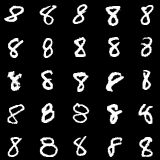
\includegraphics[width=\textwidth]{figures/einsum/8mnist_ground_truth.png}
        \caption{Ground Truth}
    \end{subfigure}
    \begin{subfigure}[b]{0.24\textwidth}
        \centering
        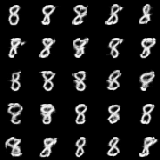
\includegraphics[width=\textwidth]{figures/einsum/8mnist_EM.png}
        \caption{EM (LL: -15984)}
    \end{subfigure}
    \begin{subfigure}[b]{0.24\textwidth}
        \centering
        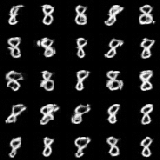
\includegraphics[width=\textwidth]{figures/einsum/8mnist_SGD.png} 
        \caption{SGD (LL: -17996)}
    \end{subfigure}
    \begin{subfigure}[b]{0.24\textwidth}
        \centering
        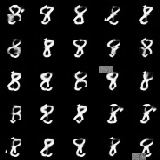
\includegraphics[width=\textwidth]{figures/einsum/8mnist_SSM.png}
        \caption{SSM (LL: -22213)}
    \end{subfigure}
    \caption{Samples and Log-Likelihood of MNIST-class 8}
\end{figure}

\begin{figure}[H]
    \centering
    \begin{subfigure}[b]{0.24\textwidth}
        \centering
        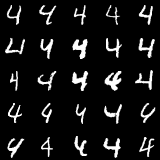
\includegraphics[width=\textwidth]{figures/einsum/4mnist_ground_truth.png}
        \caption{Ground Truth}
    \end{subfigure}
    \begin{subfigure}[b]{0.24\textwidth}
        \centering
        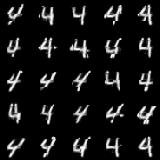
\includegraphics[width=\textwidth]{figures/einsum/4mnist_EM.png}
        \caption{EM (LL: -13131)}
    \end{subfigure}
    \begin{subfigure}[b]{0.24\textwidth}
        \centering
        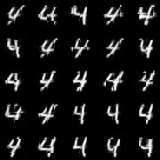
\includegraphics[width=\textwidth]{figures/einsum/4mnist_SGD.png} 
        \caption{SGD (LL: -15170)}
    \end{subfigure}
    \begin{subfigure}[b]{0.24\textwidth}
        \centering
        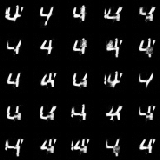
\includegraphics[width=\textwidth]{figures/einsum/4mnist_SSM.png}
        \caption{SSM (LL: -20513)}
    \end{subfigure}
    \caption{Samples and Log-Likelihood of MNIST-class 4}
\end{figure}

\begin{figure}[H]
    \centering
    \begin{subfigure}[b]{0.24\textwidth}
        \centering
        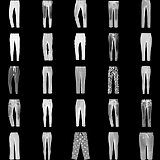
\includegraphics[width=\textwidth]{figures/einsum/1fashion-mnist_ground_truth.png}
        \caption{Ground Truth}
    \end{subfigure}
    \begin{subfigure}[b]{0.24\textwidth}
        \centering
        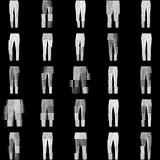
\includegraphics[width=\textwidth]{figures/einsum/1fashion-mnist_EM.png}
        \caption{EM (LL: -8230)}
    \end{subfigure}
    \begin{subfigure}[b]{0.24\textwidth}
        \centering
        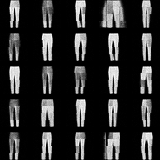
\includegraphics[width=\textwidth]{figures/einsum/1fashion-mnist_SGD.png} 
        \caption{SGD (LL: -8142)}
    \end{subfigure}
    \begin{subfigure}[b]{0.24\textwidth}
        \centering
        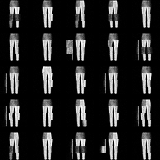
\includegraphics[width=\textwidth]{figures/einsum/1fashion-mnist_SSM.png}
        \caption{SSM (LL: -10797)}
    \end{subfigure}
    \caption{Samples and Log-Likelihood of FashionMNIST-class 1}
\end{figure}

\begin{figure}[H]
    \centering
    \begin{subfigure}[b]{0.24\textwidth}
        \centering
        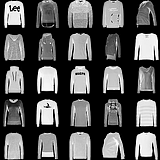
\includegraphics[width=\textwidth]{figures/einsum/2fashion-mnist_ground_truth.png}
        \caption{Ground Truth}
    \end{subfigure}
    \begin{subfigure}[b]{0.24\textwidth}
        \centering
        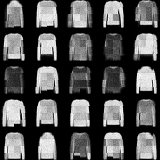
\includegraphics[width=\textwidth]{figures/einsum/2fashion-mnist_EM.png}
        \caption{EM (LL: -11973)}
    \end{subfigure}
    \begin{subfigure}[b]{0.24\textwidth}
        \centering
        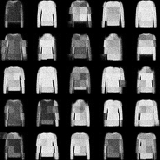
\includegraphics[width=\textwidth]{figures/einsum/2fashion-mnist_SGD.png} 
        \caption{SGD (LL: -12909)}
    \end{subfigure}
    \begin{subfigure}[b]{0.24\textwidth}
        \centering
        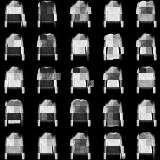
\includegraphics[width=\textwidth]{figures/einsum/2fashion-mnist_SSM.png}
        \caption{SSM (LL: -17594)}
    \end{subfigure}
    \caption{Samples and Log-Likelihood of FashionMNIST-class 2}
\end{figure}

\begin{figure}[H]
    \centering
    \begin{subfigure}[b]{0.24\textwidth}
        \centering
        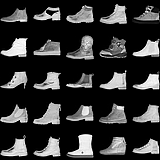
\includegraphics[width=\textwidth]{figures/einsum/9fashion-mnist_ground_truth.png}
        \caption{Ground Truth}
    \end{subfigure}
    \begin{subfigure}[b]{0.24\textwidth}
        \centering
        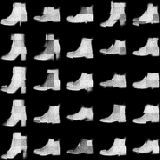
\includegraphics[width=\textwidth]{figures/einsum/9fashion-mnist_EM.png}
        \caption{EM (LL: -11173)}
    \end{subfigure}
    \begin{subfigure}[b]{0.24\textwidth}
        \centering
        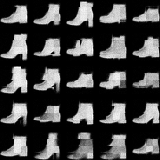
\includegraphics[width=\textwidth]{figures/einsum/9fashion-mnist_SGD.png} 
        \caption{SGD (LL: -11632)}
    \end{subfigure}
    \begin{subfigure}[b]{0.24\textwidth}
        \centering
        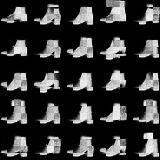
\includegraphics[width=\textwidth]{figures/einsum/9fashion-mnist_SSM.png}
        \caption{SSM (LL: -15864)}
    \end{subfigure}
    \caption{Samples and Log-Likelihood of FashionMNIST-class 9}
\end{figure}

The main findings were quite similar to the 2D Density Estimation Results. EM and SGD performed quite similar and SSM lagged a little behind. 
Also the training iterations needed and the training time reflected the 2D counterpart. 

Additionally we found, that in the samples SSM often was the least "blurry", but on the other hand SSM seemed to often only train 
one particular type of the provided digit or fashion-piece, best seen in \ref{fig:mnist7}. This happens because one weight in the mixture approaches $1$ while 
all others are at nearly $0$. \\
It is also noteworthy that EM and SGD were very robust with regard to the training parameters, they nearly always finished and produced at least reasonable results. 
SSM was very fragile especially when it came to the learning rate, where when choosing a low learning rate it took way too many iterations 
and when choosing a too high learning rate the gradients either vanished or exploded. Eventually we decided to decay the learning rate over 
the iterations but this decay process also had to be tuned for each dataset. 